% Pieds de page pour les pages de chapitre
\thispagestyle{empty}

\setstretch{1}

\begin{center}
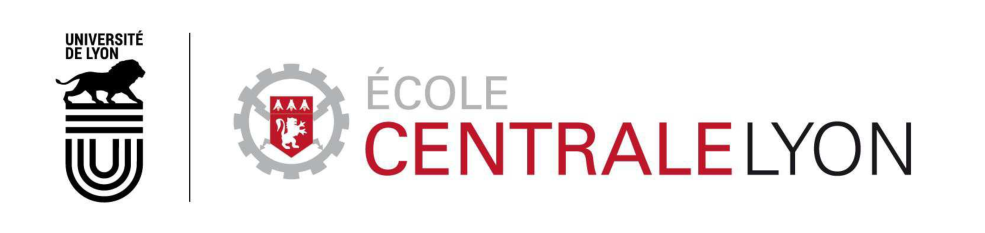
\includegraphics[width=0.99\linewidth]{logo_UDL.eps}
\end{center}
N$^\circ$ d'ordre NNT: 1966LYSEC??
\vskip 2cm
\begin{center}
\textbf{\Large{TH\`ESE de DOCTORAT DE L'UNIVERSIT\'E DE LYON}}\\
\textbf{\Large{opérée au sein de l'\'Ecole Centrale de Lyon \\[3ex]
\'Ecole Doctorale N$^\circ$ 162}} \\
\textbf{\large{Mécanique \'Energétique Génie Civil Acoustique\\[3ex]
Spécialité de doctorat : Acoustique}} \\[5ex]
{\large{Soutenue publiquement le 16/12/1966, par \\[1ex]
\textbf{Monsieur Spock} }}
\end{center}

\vskip 8ex

\noindent
\rule{\textwidth}{1pt}

\begin{center}
{\LARGE{}
\textbf{Scientific Essay on the Theory of Everything}
\\}
\end{center}
\noindent
\rule{\textwidth}{1pt}
\vskip 2cm
\noindent \hspace{-0.5cm} Devant le jury composé de
\vskip 0.5cm
\begin{tabbing}
\hspace{-0.5cm}\=\hspace{4.3cm}\=\hspace{2.2cm}\=\hspace{7.6cm}\=\kill
\> Kolmogorov, Andreï\> Professeur \> Université d'État de Moscou \> Directeur de thèse\\  
\> Landau, Lev Davidovitch\> Professeur \> Université de Kharkov \> Rapporteur\\ 

\end{tabbing} 
